\documentclass{standalone}
\usepackage{amsfonts, amsmath, amssymb, bm} %Math fonts and symbols
\usepackage{dcolumn, multirow} % decimal-aligned columns, multi-row cells
\usepackage[colorlinks=true]{hyperref}
\usepackage{graphicx, subfigure, float} % graphics commands
\usepackage[margin=1in]{geometry} % sets page layout
\usepackage{setspace}% allows toggling of double/single-spacing
\usepackage{verbatim}% defines environment for un-evaluated code
\usepackage{natbib}% defines citation commands and environments.
\singlespace % set document spacing to single
\bibpunct[, ]{(}{)}{,}{a}{}{,} % sets the punctuation of the bibliography entires.
\newcolumntype{d}[1]{D{.}{.}{#1}} % defines a decimal-aligned column
\usepackage{tikz}
\usetikzlibrary{intersections}
\usepackage{enumerate}
\usepackage[utf8]{inputenc}
\usepackage[english]{babel}
\hyphenpenalty=10000

\begin{document}
    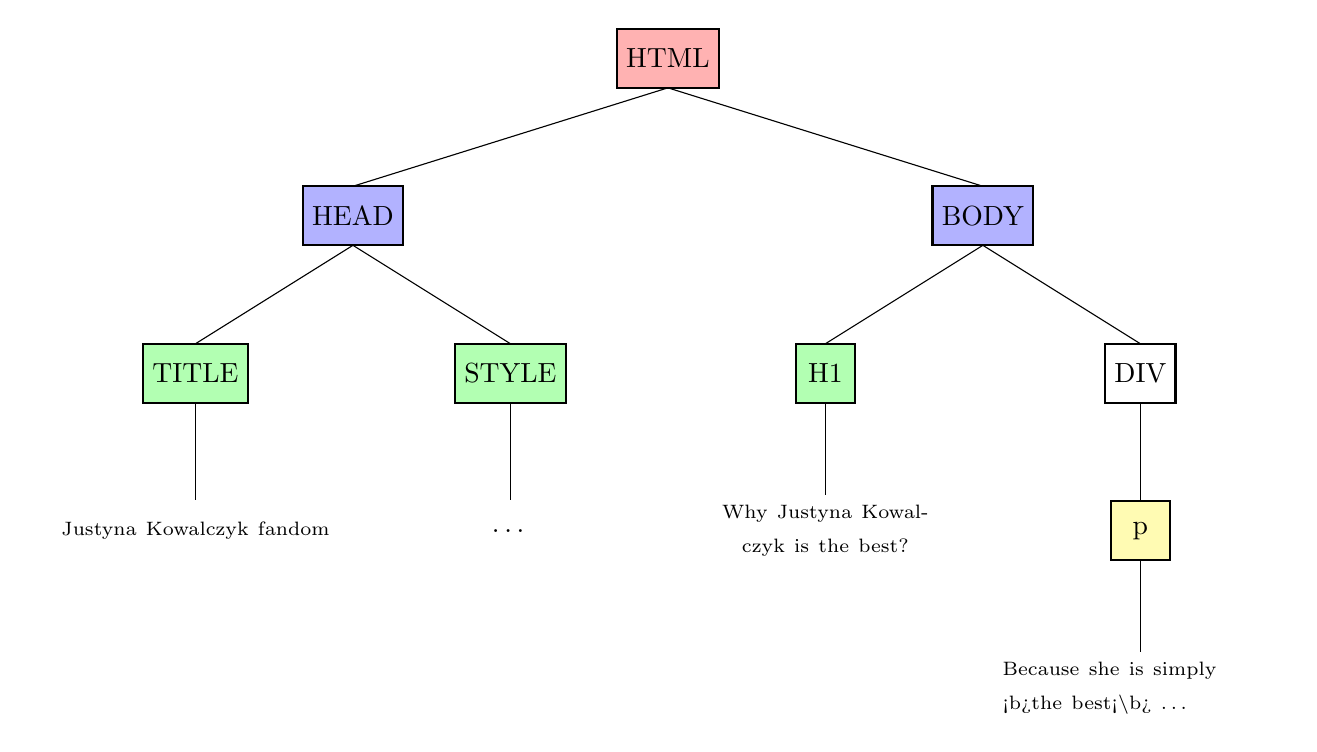
\begin{tikzpicture}[>=stealth, small/.style={
		% The shape:
		rectangle,
		% The size:
		minimum size=.75cm,
		% The border
		thick, draw=black,
		% The filling
		fill=white}]
    \node [small, fill = red!30] at (0,0) {HTML};
    \draw (0,-.375) -- (-4,-1.625);
    \draw (0,-.375) -- (4,-1.625);
    \node [small, fill = blue!30] at (-4,-2) {HEAD};
    \draw (-4, -2.375) -- (-6, -3.625);
    \draw (-4, -2.375) -- (-2, -3.625);
    \node [small, fill = green!30] at (-6, -4) {TITLE};
    \draw (-6, -4.375) -- (-6, -5.625);
    \node [small, draw=white, text width = 4cm, align = center] at (-6, -6) {\scriptsize Justyna Kowalczyk fandom};
    \node [small, fill = green!30] at (-2, -4) {STYLE};
    \draw (-2, -4.375) -- (-2, -5.625);
    \node [small, draw=white] at (-2, -6) {\dots};
    \node [small, fill = blue!30] at (4,-2) {BODY};
    \draw (4, -2.375) -- (6, -3.625);
    \draw (4, -2.375) -- (2, -3.625);
    \node [small, fill = green!30] at (2, -4) {H1};
    \draw (2, -4.375) -- (2, -5.625);
    \node [small, draw=white, text width = 3.5 cm, align = center] at (2, -6) {\scriptsize Why Justyna Kowalczyk is the best?};
    \node [small] at (6, -4) {DIV};
    \draw (6, -4.375) -- (6, -5.625);
    \node [small, fill=yellow!30] at (6, -6) {p};
    \draw (6, -6.375) -- (6, -7.625);
    \node [small, draw=white, text width = 3.5cm] at (6, -8) {\scriptsize Because she is simply <b>the best<$\backslash$b> \dots};
    \end{tikzpicture}
\end{document}
